\documentclass[a4paper, 12pt]{article}

\usepackage[utf8]{inputenc}
\usepackage[T1]{fontenc}
\usepackage[english]{babel}
%\usepackage{layout}
\usepackage[top=3cm, bottom=3cm, left=2.5cm, right=2.5cm]{geometry}\usepackage{setspace} %interligne
%\usepackage{soul}
%\usepackage{ulem}
%\usepackage{eurosym}
%\usepackage{bookman}
%\usepackage{charter}
%\usepackage{newcent}
%\usepackage{lmodern}
%\usepackage{mathpazo}
%\usepackage{mathptmx}
%\usepackage{url}
\usepackage{graphicx}
\usepackage{verbatim}
%\usepackage{moreverb}
%\usepackage{listings}
\usepackage{fancyhdr}
%\usepackage{wrapfig}
%\usepackage{color}
%\usepackage{colortbl}
\usepackage{amsmath}
\usepackage{amssymb}
\usepackage{mathrsfs}
%\usepackage{asmthm}
%\usepackage{makeidx}
\usepackage{lastpage}
\usepackage{float}

\usepackage{listings}
\lstset{
language=MATLAB,
basicstyle=\footnotesize,
numberstyle=\normalsize,
numbersep=7pt,
}

\pagestyle{fancy}

\renewcommand\headrulewidth{1pt}
\fancyhead[L]{Zaki Chaïr \& Alexandre Ladrière - EI17}
\fancyhead[R]{M\&S - Caractérisation sécuritaire}
\renewcommand\footrulewidth{1pt}
\fancyfoot[C]{
\textbf{Page \thepage/\pageref{LastPage}}}

\onehalfspacing

\title{\huge{\begin{bf} Réalisation pratique d'attaques\end{bf}} \\ \begin{doublespacing} \large{Caractérisation sécuritaire par analyse du rayonnement EM} \end{doublespacing} \vspace{\fill}}
\author{Zaki CHAIR \& Alexandre LADRIERE}
\date{Janvier 2020}

\begin{document}

	\begin{figure}
	\begin{center}
	
\includegraphics[scale=0.5]{images/emse_logo.png}
	\end{center}
	\end{figure}

\maketitle\thispagestyle{empty}
\newpage
\tableofcontents
\newpage

\section{Introduction}
La caractérisation sécuritaire par canaux cachés repose sur une analyse statistique du champ électromagnétique ou de la consommation du circuit pendant son fonctionnement.
L'objectif de ce TP était de mettre en évidence l'attaque par analyse de champ EM correspondant à l'exécution d'une implantation logicielle de l'algorithme de chiffrement AES 128-bits sans protections, sur un microcontrôleur 8 bits, non sécurisé. Ce TP est lui-même décomposé en plusieures parties. 

Dans la première partie, nous devions analyser et comprendre le principe de l'attaque sur cette cible. Nous devions également valider le set-up d'acquisition permettant de mesurer un rayonnement exploitable par l'analyse statistique. Dans la deuxième partie, nous devions faire un certain nombre de relevés du champ EM puis élaborer un script Matlab permettant de retrouver la clé initiale utilisée dans l'AES à partir de ces relevés. Il s'agit de l'analyse statistique. La troisième partie concernait l'analyse des résultats obtenus et l'influences des divers paramètres sur le crackage de clé. Enfin, la dernière partie concernait les contre-mesures softwares qu'il était possible de mettre en place. 
\newpage
\section{Première partie: Validation du set-up}
	\subsection{Principe de l'attaque par analyse des champs EM}
	L'attaque par analyse des champs EM consiste à capturer les rayonnements EM d'une cible exécutant un algorithme de chiffrement afin de pouvoir récupérer certaines informations et ainsi remonter à la clé de chiffrement qui constitue le secret. Il s'agit d'une attaque non invasives et passive (observation du comportement de la cible sans dommage physique sur la cible, mais les résultats restes plus précis si on dépackage la cible). 
	
	Des ondes électromagnétiques sont émises lors de la circulation d'un courant dans les transistors présents dans la cible. De plus, le champ EM est directement dépendant de l'intensité circulant dans ces transistors, par la relation suivante:
	\begin{align*}
		Champs EM \;\; = \;\; \frac{di}{dt} \;\; , \;\; \textrm{avec i l'intensité}
	\end{align*}
Or, la consommation électrique varie en fonction des opérations effectuées. Ainsi, on aura une variation du champ EM en fonction des opérations effectuées, et donc obtenir des informations pour remonter à la clé initiale. 

	\subsection{Détermination de la cible de l'attaque dans l'algorithme}
	L'algorithme implémenté sur la cible est un AES 128 bits. Cet algorithme se décompose en quatre transformations élémentaires: \emph{AddRoundKey}, \emph{SubBytes}, \emph{MixColumns} et \emph{ShiftRows}. L'algorithme se déroule en 11 rondes: 1 ronde initiale, suivie de 9 rondes éxecutant les 4 fonctions citées précédemment, et une dernière ronde ne faisant pas intervenir \emph{MixColumns}, comme illustré en figure~\ref{AES_principe}.
	
	Un bloc de données sur 16 octets (i.e. 128 bits) forme le message à chiffrer en entrée de l'algorithme. Une clé secrète utilisée lors de la ronde initiale et dérivée ensuite dans les rondes suivantes constitue le secret de cet algorithme. Une fonction nommée \emph{KeyExpansion} est utilisée pour générer les clés de rondes à partir de la clé initiale. 

		\begin{figure}[H]
			\begin{center}
			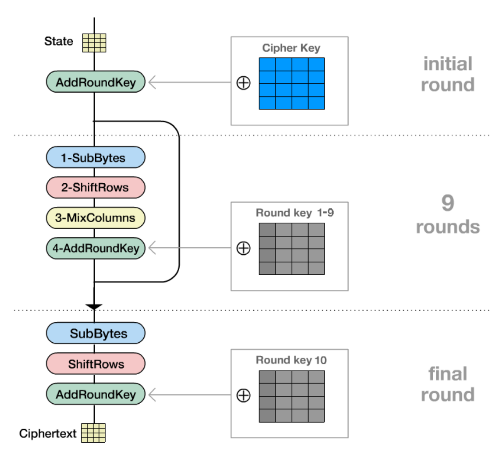
\includegraphics[scale=0.7]{images/AES_principe.png}
			\end{center}
			\caption{Fonctionnement du chiffrement pour AES-128}
			\label{AES_principe}
		\end{figure}

Dans notre cas, nous connaissons le \emph{plain text} utilisé lors du chiffrement, et nous voulons remonter à la clé initiale. Or, la clé initiale est utilisée lors du premier \emph{SubBytes} (ronde 0). Ainsi, nous allons nous focaliser sur la ronde 1. 
De plus, nous cherchons une fonction non linéaire afin d'avoir le maximum de variations de courant (une fonction linéaire implique peu de transitions de bits, et donc peu de variations d'intensité électrique). \textbf{C'est pourquoi nous allons cibler le \emph{SubBytes} de la ronde 1}. En effet, \emph{SubBytes} n'est pas linéaire à cause de l'utilisation de la S-Box.

	\subsection{Acquisition du champs EM}
	Pour réaliser cette étape nous disposions des éléments suivants:
	\begin{itemize}
		\item Oscilloscope de la famille Picoscope
		\item Sonde électromagnétique Langer
		\item PC servant d'unité de commande
		\item Amplificateur Langer P303A
		\item Carte de développement STM32F0
		\item Convertisseur USB-RS232 pmod232
		\item Keil Vision: développement de l'AES 128-bis
		\item ST-Link: transfert du binaire vers la cible
		\item Programme de validation de la communication du PC vers la cible
		\item Programme d'acquisition de traces EM
	\end{itemize}
	
	Nous avons dans un premier temps transféré le binaire du code AES 128-bits sur la cible, puis vérifié son fonctionnement (la trace de ce test est disponible en annexe~\ref{test_results} page~\pageref{test_results}, ainsi que la clé initiale utilisée dans le code en annexe~\ref{init_key} page~\pageref{init_key})

Une fois que nous avons vérifié le bon fonctionnement de l'AES, nous avons modifié ce code afin de déclencher un signal de trigger pour le \emph{SubBytes} de la ronde 1 en mettant à 1 le GPIO 8 du port B au début du \emph{SubBytes}, et en le repassant à 0 à la fin de cette opération:
\begin{lstlisting}
****************************************************************
void AES_Run(void)
{
  int i;
  addRoundKey();
  for(i = 0; i < 9; i++)
  {
    if(i==0)
    {
      // trigger sur le premier SubBytes
      GPIOB->BSRR = GPIO_Pin_8;
      subBytes();
      GPIOB->BRR = GPIO_Pin_8;
    }
    else
    {
      subBytes();		
    }
    shiftRows();
    mixColumns();
    computeKey(rcon[i]);
    addRoundKey();
  }
  subBytes();
  shiftRows();
  computeKey(rcon[i]);
  addRoundKey();
}
****************************************************************
\end{lstlisting}

Ce trigger nous permet de visualiser le premier \emph{SubBytes} lors de la mesure du champs EM. 

Ensuite, nous avons observé le champ EM sur l'opération ciblé, et nous avons déplacé la sonde EM au-dessus du microcontrôleur et au plus près de celui-ci afin de réduire au maximum le bruit (en effet, l'information obtenue peut être plus ou moins bruitée par les calculs réalisés en parallèle par le circuit ou par des signaux externes).

Puis, nous avons lancé le chiffrement en continu, afin de visualiser au mieux l'étape cible et ainsi de visualiser correctement le champ EM émit lors de cette étape. Nous obtenons alors le champ représenté en figure~\ref{subbytes_capture_pico}.
		\begin{figure}[H]
			\begin{center}
			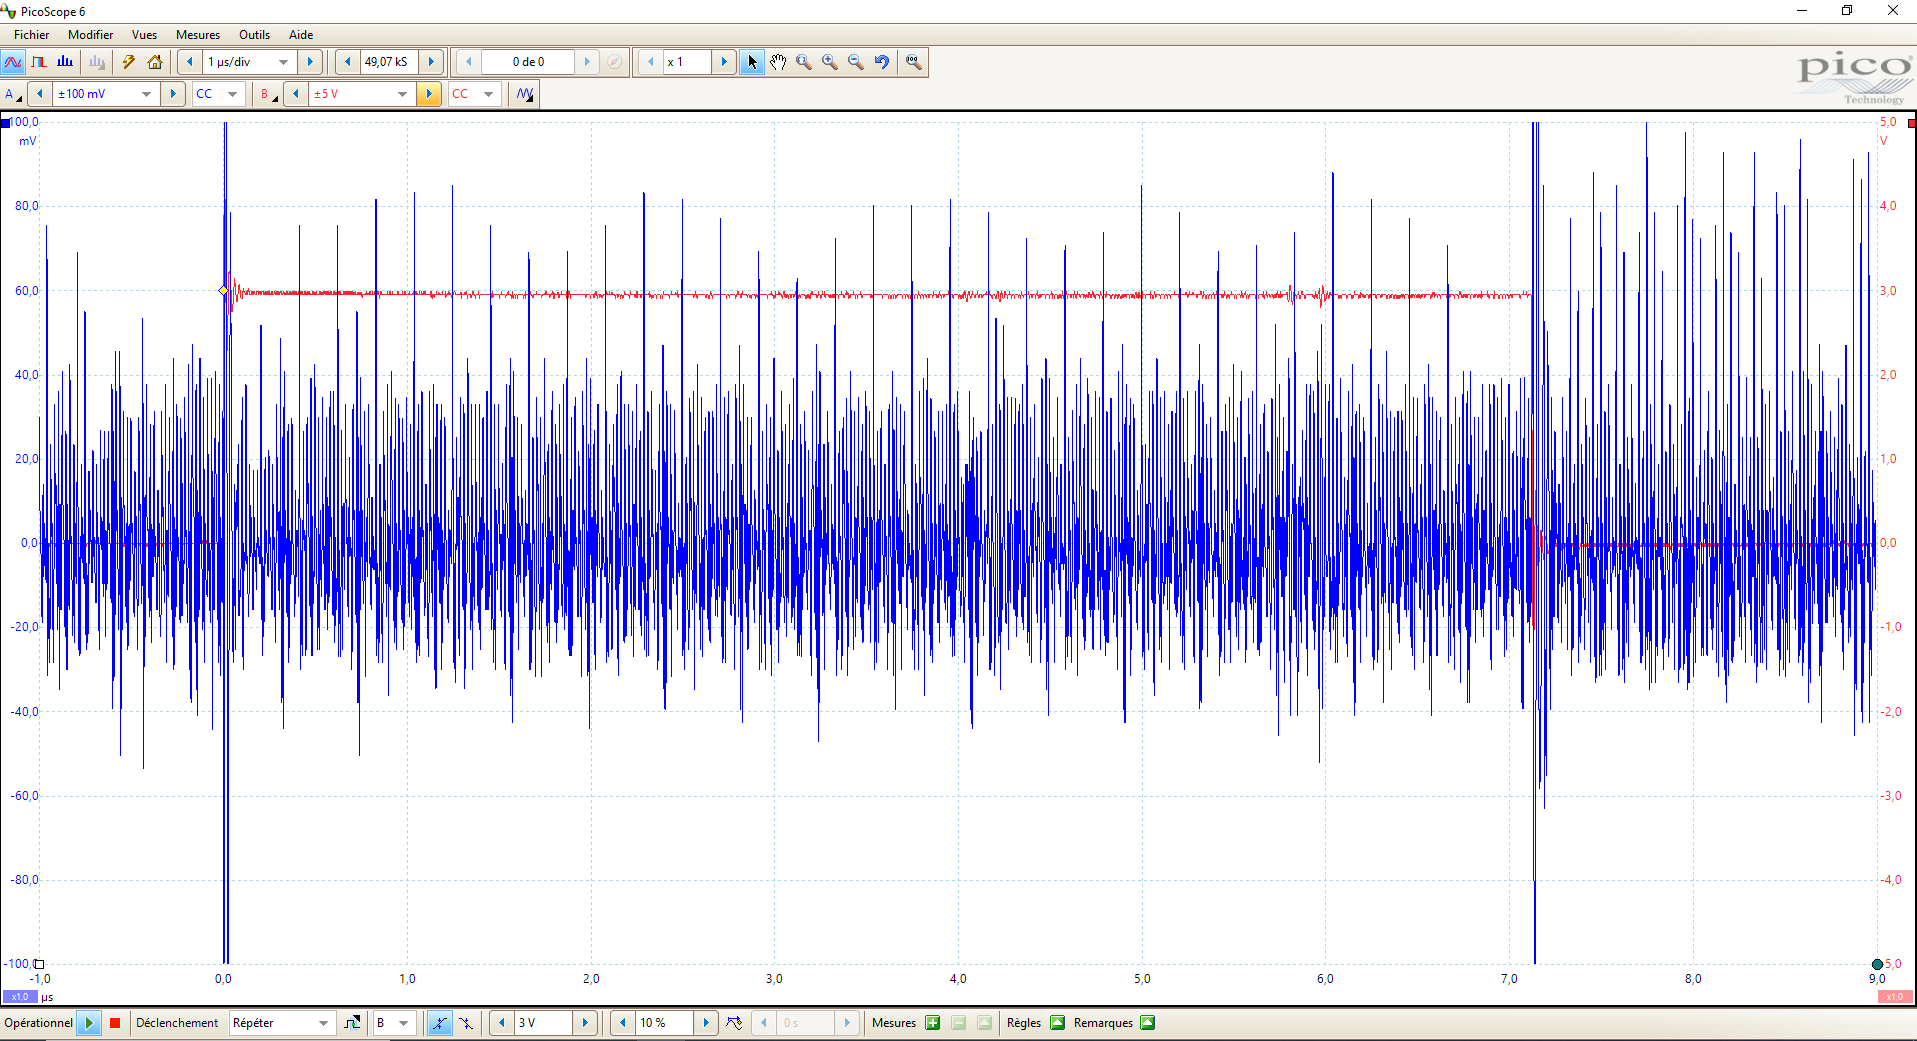
\includegraphics[scale=0.3]{images/subbytes_capture_pico.PNG}
			\end{center}
			\caption{Capture du champs EM émis lors du \emph{SubBytes} de la ronde 1}
			\label{subbytes_capture_pico}
		\end{figure}

\newpage
\section{Deuxième partie: Acquisition et analyse statistique}
	\subsection{Acquisition du champ EM}
	Afin de relever les traces du champ EM, nous avons utilisé la même disposition que précédemment. Cependant, cette fois nous avons, grâce à un script, effectué le relevé du champ EM (au format \emph{.mat}) pour 300 plain text différents. 
	
Par exemple, pour le plain text suivant:
\begin{lstlisting}
36 33 f1 e7 14 7b c0 67 44 5d 6b 5d e5 67 7b d4
\end{lstlisting}
nous obtenons le relevé de la figure~\ref{matlab_trace_1}.
		\begin{figure}[H]
			\begin{center}
			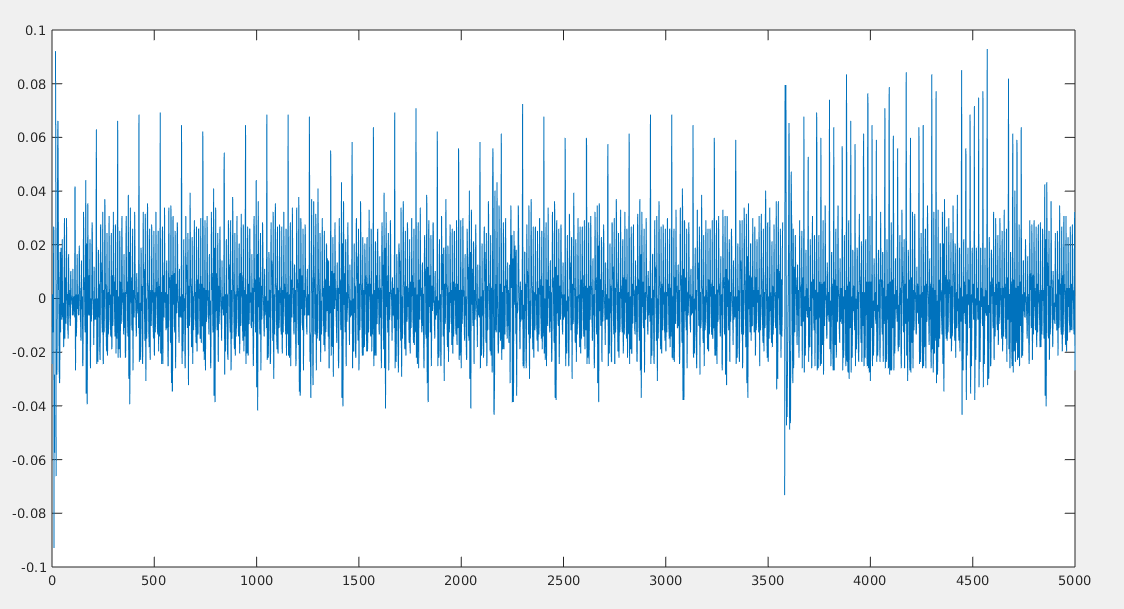
\includegraphics[scale=0.3]{images/matlab_trace_1.png}
			\end{center}
			\caption{Trace du champ EM émis lors du \emph{SubBytes} de la ronde 1}
			\label{matlab_trace_1}
		\end{figure}
		
	\subsection{Analyse statistique}
	Maintenant que nous disposons de ces 300 traces du champ EM correspondant à l'activité de la fonction \emph{SubBytes} de la ronde 1, nous pouvons procéder à l'analyse statistique dite CEMA pour \emph{Correlation Electro-Magnetic Analysis}. Cette analyse sera effectué grâce à un script Matlab (disponible en annexe~\ref{Script_Matlab} page~\pageref{Script_Matlab}).
	
	Afin de retrouver la clé utilisée, la première étape consiste à prédire la consommation à la sortie de cette fonction. La prédiction est calculée selon un modèle de fuite en utilisant le poids de Hamming (\emph{Hamming Weight}). Il est simple à implémenter car il suffit de calculer le nombre de '1' en sortie de la fonction \emph{SubBytes}.
	
	\subsubsection{Etape 1: construction de la matrice des traces}
		La première étape dans notre script consiste à regrouper toutes les traces (déjà au format \emph{.mat}) dans une seule et même matrice. Cette matrice, nommée $matrix\_trace$ est de taille $300$ x $5000$. En effet, nous avons effectué 300 relevés, et chaque relevé comporte 5000 points. Chaque ligne de cette matrice correspond à un relevé de champ EM. Voici la fonction effectuant cette opération:\\
		
\begin{lstlisting}
****************************************************************
function mat = getTraces(path, p_nb_trace, p_nb_points)
    % Load all the matrix traces in a global matrix (and switch 
    % lines to columns)
    mat = zeros(p_nb_trace, p_nb_points);
    for i=1:p_nb_trace
        path_current_trace = append(path, 'Trace (', int2str(i), ').mat');
        T = load(path_current_trace, '-mat');
        for j=1:p_nb_points
            mat(i,j) = T.A(j, 1);
        end
    end
end
****************************************************************
\end{lstlisting}

		\subsubsection{Etape 2: construction de la matrice des plain text}
		La seconde étape consiste à récupérer tous les plain texts utilisées dans une matrice de taille $300$ x $16$ (chaque plain text a une longueur de 16 octets. Voici la fonction effectuant cette opération:\\
\begin{lstlisting}
****************************************************************
function mat = getPlainText(p_ptext_path, p_nb_trace, p_nb_bytes)
    % Load the plain text (hex format) in a matrix (dec format)
    mat = zeros(p_nb_trace, p_nb_bytes);
    fid = fopen(p_ptext_path);
    for i = 1:p_nb_trace
        tline = fgetl(fid); % current line
        % split current line each 2 characters, e.g. 
        % "0A22FF1C" will become ['0A' '22' 'FF' '1C']
        tmp_line = cellstr(reshape(tline,2,[])'); 
        for j = 1:p_nb_bytes
            mat(i, j) = hex2dec(tmp_line(j));
        end
    end
end
****************************************************************
\end{lstlisting}

		\subsubsection{Etape 3: Hypothèses de consommation}
		La troisième étape consiste à effectuer les hypothèses de consommation à un instant donnée pour chaque valeur de clé possible. 
		Imaginons que nous souhaitons faire une hypothèse de consommation pour déterminer l'octet $X$ de la clé. Alors, pour chacune des 256 valeurs possibles de clé (\emph{0x00} à \emph{0xFF}) on va effectuer un \emph{XOR} entre cette valeur $K$ et la valeur $P$ correspondant à l'octet en position $X$ de chaque plain text:
		\begin{align*}
		R \;\; = \;\; K \;\; \oplus \;\; P
		\end{align*}
Ensuite, on va chercher dans la S-Box la valeur correspondant à ce $R$. Ensuite, le poids de Hamming $H$ est calculé pour la valeur récupérée dans la S-Box. Puis, ce poids est mis dans une nouvelle matrice, $matrix\_hamming$ de taille $256$ x $300$. Chaque ligne de cette matrice correspond aux poids de hamming pour chaque octet en position $X$ des plain texts pour une valeur de clé $K$ donnée. 

A la fin de ces boucles (position $X$ fixée), nous avons une matrice d'hypothèse que nous pouvons utiliser dans l'étape suivante. 
\textbf{FAIRE SCHEMA}
Voici le code utilisé pour réaliser cette étape:
\begin{lstlisting}
****************************************************************
for i = 1:p_nb_bytes
        for j = 0:255
            for k = 1:p_nb_trace 
                xor = bitxor(j, p_matrix_plain_text(k,i));
                out_sbox = p_sbox(xor + 1); % +1 because arrays start 1...
                hamming_weight = sum(dec2bin(out_sbox).' == '1'); % Hamming weight
                mat_hamming(j+1, k) = hamming_weight;
            end
        end 
        % at this point we have the hamming weight matrice 
        % for one column in the plain text file (i.e. the line 
        % are for key hypethosis, and the column for a specific trace)
end
****************************************************************
\end{lstlisting}

			\subsubsection{Etape 4: Détermination de la clé}
		L'étape suivante consiste à calculer la matrice de corrélation. Cela signifie que l'on crée une nouvelle matrice, $matrix\_correlation$ de taille $256$ x $5000$, ou chaque indice $(i, j)$ correspond au coefficient de corrélation entre la ligne $i$ de $matrix\_hamming$ et la colonne $j$ de $matrix\_traces$.
Voici le code permettant de faire cela:
\begin{lstlisting}
****************************************************************
for i = 1:p_nb_bytes
	for m = 1:p_nb_points
    	for n = 0:255
        	[r,p] = corrcoef(mat_hamming(n+1, :), p_matrix_traces(:, m));
            corr_factor = r(2, 1);
            mat_corr(n+1,m) = corr_factor;
        end
    end
end
****************************************************************
\end{lstlisting}


Ensuite, pour trouver l'octet de clé correspondante, il suffit de rechercher l'indice de ligne du maximum de $matrix\_correlation$. 
\begin{lstlisting}
****************************************************************
% find the maximum value in the matrix
maximum = max(max(mat_corr)); 
% get the coordinates (line, column) of the maximum value
[x, y] = find(mat_corr == maximum); 
hyp_key = append(hyp_key, " ", dec2hex(x-1, 2)); % -1 because array starts at 1
****************************************************************
\end{lstlisting}


Après avoir effectué ce principe pour chaque octet de la clé, notre script écrit la clé finale dans un fichier texte accompagné des facteurs de corrélation pour chaque octet. Voici ce que nous avons obtenus:
\begin{lstlisting}
Key: 17 9E 48 16 28 AE D2 A6 AB F7 15 88 09 CF 4F 3C


KEY 	CORR_COEF
 	 
17 	 0.60015
9E 	 0.60564
48 	 0.65908
16 	 0.58929
28 	 0.6158
AE 	 0.72205
D2 	 0.6304
A6 	 0.51066
AB 	 0.46422
F7 	 0.5488
15 	 0.5295
88 	 0.56779
09 	 0.46489
CF 	 0.57992
4F 	 0.51666
3C 	 0.6416
\end{lstlisting}

Cela correspond bien à la clé utilisée par l'AES lors de nos 300 relevés de champ EM:
\begin{lstlisting}
void AES_InitKey()
{
	key[0]=0x17;
	key[1]=0x9e;
	key[2]=0x48;
	key[3]=0x16;
	key[4]=0x28;
	key[5]=0xae;
	key[6]=0xd2;
	key[7]=0xa6;
	key[8]=0xab;
	key[9]=0xf7;
	key[10]=0x15;
	key[11]=0x88;
	key[12]=0x09;
	key[13]=0xcf;
	key[14]=0x4f;
	key[15]=0x3c;
}
\end{lstlisting}


\textbf{FAIRE SCHEMA GLOBAL CF. TABLEAU}


\newpage
\section{Troisième partie: Analyse des résultats}
	\subsection{Position de la fuite par octets}
Afin de visualiser la position des fuites pour chaque octes, nous avons également relevé l'indice de colonne du maximum de $matrix\_correlation$, en plus de l'indice de ligne (qui correspondait à la valeur de l'octet de la clé). En superposant la trace d'un champ EM et ces points sur le même graph, nous obtenons la figure~\ref{leak_time}, où les droites verticales rouges représentent l'endroit où le maximum de corrélation a été trouvé pour chaque octet.

\begin{figure}[H]
	\begin{center}
		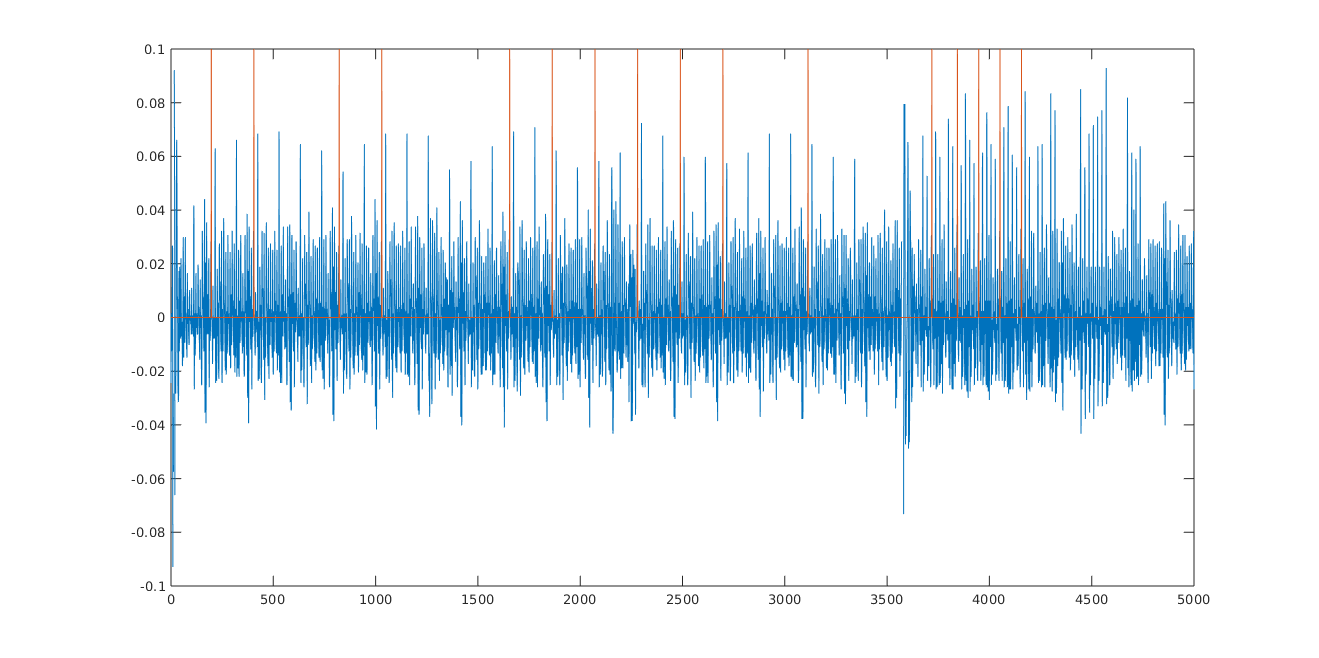
\includegraphics[scale=0.4]{images/leak_time.png}
		\caption{Superposition de la position des fuites et d'un champ EM}
		\label{leak_time}
	\end{center}
\end{figure}	
	
	En observant cette figure, on remarque que les instants où le maximum de corrélation (et donc l'octet de la clé) ont été trouvé ne sont pas tous dans la zone associée au \emph{SubBytes} (cf. figure~\ref{subbytes_capture_pico} page ~\pageref{subbytes_capture_pico}).
	
	Nous avons donc refait tourner notre script, mais cette fois en limitant la zone d'étude aux 3500 premiers points (ce qui correspond à l'étape \emph{SubBytes}). On obtient alors les résultats suivants:
\begin{lstlisting}
Key:  17 9E 48 16 28 AE D2 A6 AB F7 15 88 09 CF 4F 3C


KEY  CORR_COEF
 	 
17 	 0.60015
9E 	 0.60564
48 	 0.60468
16 	 0.58929
28 	 0.6158
AE 	 0.46858
D2 	 0.5406
A6 	 0.51066
AB 	 0.46422
F7 	 0.5488
15 	 0.5295
88 	 0.56779
09 	 0.46489
CF 	 0.56971
4F 	 0.51666
3C 	 0.50886
\end{lstlisting}
Ainsi, nous trouvons bien la bonne clé. En tracant les instant où le maximum de corrélation a été trouvé, nous obtenons la figure~\ref{reduction_3500_pts}.

\begin{figure}[H]
	\begin{center}
		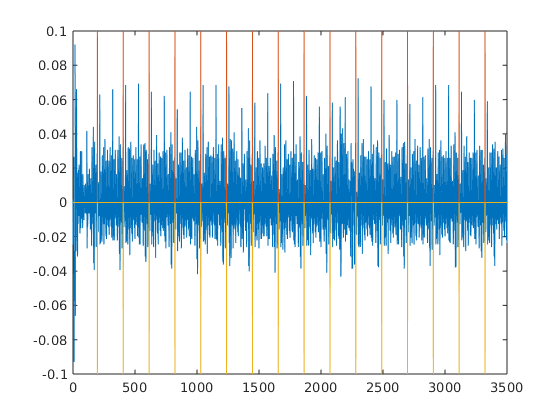
\includegraphics[scale=1]{images/reduction_3500_pts.png}
		\caption{Superposition de la position des fuites et d'un champ EM sur l'étape \emph{SubBytes}}
		\label{reduction_3500_pts}
	\end{center}
\end{figure}

Afin de valider l'importance de cibler toute la fonction \emph{SubBytes}, nous avons executé à nouveau notre script, mais cette fois avec seulement 2500 points afin de ne prendre qu'une partie de la fonction \emph{SubBytes}. Nous avons alors obtenus le résultat suivant:
\begin{lstlisting}
Key:  17 9E 48 16 28 AE D2 A6 AB F7 15 88 9C D5 66 17


KEY  CORR_COEF
 	 
17 	 0.60015
9E 	 0.60564
48 	 0.60468
16 	 0.58929
28 	 0.6158
AE 	 0.46858
D2 	 0.5406
A6 	 0.51066
AB 	 0.46422
F7 	 0.5488
15 	 0.5295
88 	 0.56779
9C 	 0.24322
D5 	 0.26025
66 	 0.25802
17 	 0.26766
\end{lstlisting}
Et le graph de localisation nous donne la figure~\ref{reduction_2500_pts}.
\begin{figure}[H]
	\begin{center}
		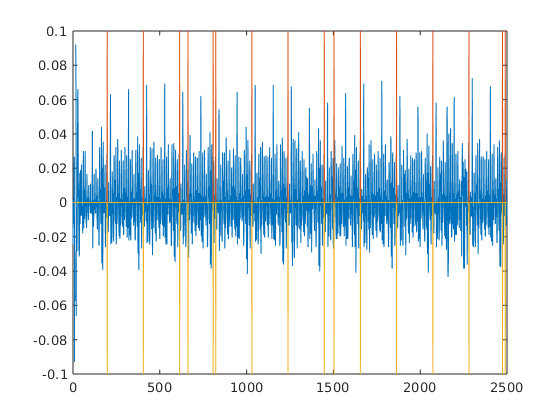
\includegraphics[scale=1]{images/reduction_2500_pts.png}
		\caption{Superposition de la position des fuites et d'un champ EM sur une partie de l'étape \emph{SubBytes}}
		\label{reduction_2500_pts}
	\end{center}
\end{figure}
Ainsi, la clé n'est pas la bonne pour les 4 derniers octets, qui sont normalement déterminés sur la partie manquant des traces ici (on peut également noter les valeurs des coefficients pour ces 4 derniers octets).
	
	\subsection{Attaque avec seulement 20 traces}
	Avec 20 traces, on obtient les résultats suivants:
\begin{lstlisting}
Key:  ED 32 E4 A2 A4 DE 4B C2 C0 AD FD 66 D7 97 DC 3C


KEY  CORR_COEF
 	 
ED 	 0.8704
32 	 0.8477
E4 	 0.84454
A2 	 0.84568
A4 	 0.85702
DE 	 0.87675
4B 	 0.84991
C2 	 0.8474
C0 	 0.85487
AD 	 0.86229
FD 	 0.87147
66 	 0.8276
D7 	 0.85549
97 	 0.83749
DC 	 0.83121
3C 	 0.84954
\end{lstlisting}

On remarque que cela ne correspond pas du tout à la clé utilisée par l'AES (c.f. ~\ref{init_key} page ~\pageref{init_key}), seul le dernier octet correspond bien à la clé recherchée, malgré la valeur élevée des coefficients de corrélation. Cela permet de bien mettre en évidence que l'utilisation seule des coéfficients de corrélation n'est pas suffisante pour déterminer la clé secrète. 
		
	\subsection{Détermination du nombre de traces minimum requises}

Nous avons fait tourner notre script pour plusieurs valeurs de nombre de traces. A chaque fois, la moyenne des coefficients de corrélation des 16 octets de la clé a été calculé. Nous avons pu obtenir le tableau~\ref{tab_corr_avg_evol}.

\begin{table}[H]
				\begin{center}
				\begin{tabular}{|c|c|c|}
					\hline
					Nombre de traces & Moyenne des coefficients de corrélation & Status clé \\
					\hline
					10 & 0.9763 & NOK (16 octets différents) \\
					\hline
					20 & 0.851835 & NOK (15 octets différents) \\
					\hline
					50 & 0.663969375 & NOK (6 octets différents) \\
					\hline
					100 & 0.5841125 & NOK (2 octets différents) \\
					\hline
					150 & 0.590869375 & OK \\
					\hline
					200 & 0.588908125 & OK \\
					\hline
					250 & 0.580720625 & OK \\
					\hline
					300 & 0.577903125 & OK \\
					\hline
				\end{tabular}
				\caption{Tableau des moyennes des coefficients de corrélation en fonction du nombre de traces}
				\label{tab_corr_avg_evol}
				\end{center}
			\end{table}

En tracant ces données, on obtient le graph de la figure~\ref{corr_avg_evol}.

		\begin{figure}[H]
			\begin{center}
			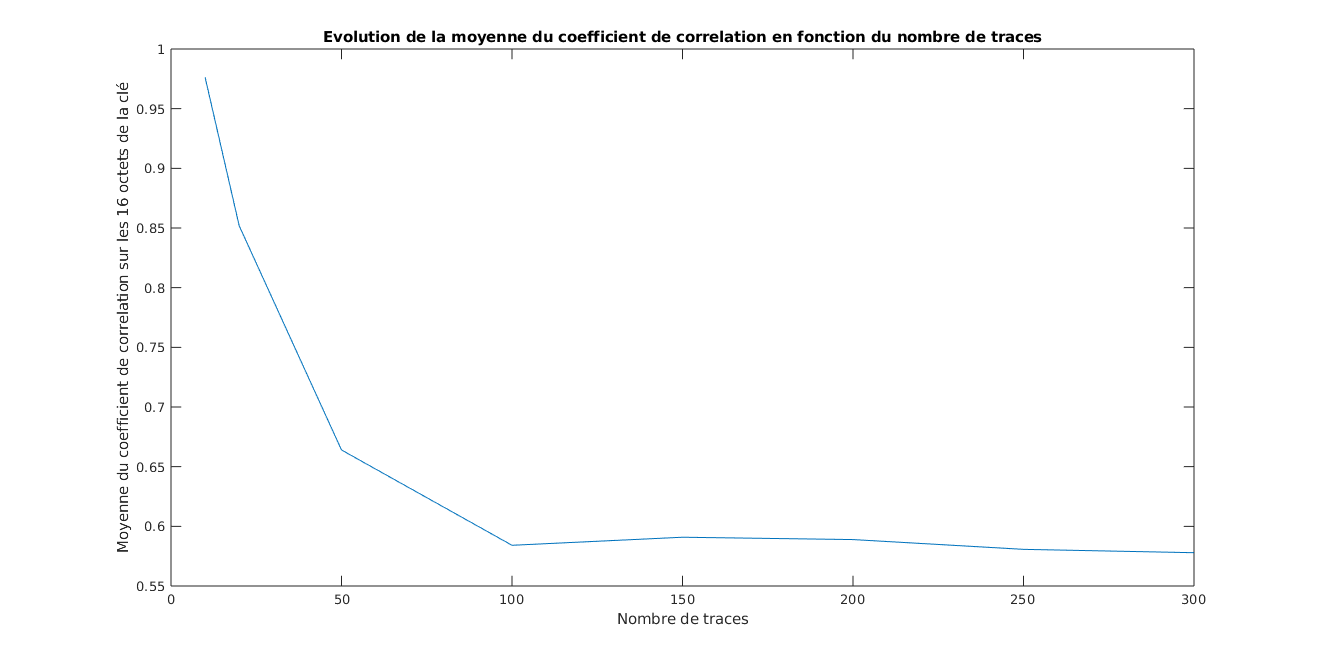
\includegraphics[scale=0.5]{images/corr_avg_evol.png}
			\end{center}
			\caption{Evolution de la moyenne des coefficients de corrélation sur les 16 octets de la clé en fonction du nombre de traces utilisées}
			\label{corr_avg_evol}
		\end{figure}

On remarque la moyenne du coefficient de corrélation se stabilise à partir d'un certains nombre de traces (environ 100). Cela correspond aussi au nombre à partir duquel on obtient la bonne clé. Ainsi, au vu de ces résultats, on estime qu'\textbf{il faut au moins 120 traces} pour obtenir la bonne clé. Ce graph, corrélé au tableau précedent, illustre bien que l'utilisation seule des coefficients de corrélation n'est pas suffisante pour déterminer la clé utilisée. 

De plus, même si l'on ne dispose que de 100 traces, il est possible d'obtenir la clé secrète en utilisant la technique de brute force pour les octets manquants (après avoir fait une analyse pour déterminer quels étaient les octets faux). En effet, il suffit d'au moins 7 bons octets pour déterminer le reste de la clé par brute force dans un temps raisonnable de nos jours. 

\section{Quatrième partie: Contre-mesures}
	On peut envisager plusieurs solutions de contre-mesures d'un point de vue software pour compliquer la vie de l'attaquant. 
	On peut par exemple, introduire de l'aléa dans le temps de calcul de \emph{SubBytes} et ainsi ne pas avoir des triggers constants autour de cette fonction. Cependant, en analysant les traces, l'attaquant se rendrait compte de cette contre-mesure et pourrait la contrer en utilisant une gaussienne et ainsi ne garder que certains paquets de courbe pour son attaque. 
	On peut également envisager d'ajouter de l'aléa dans le calcul en lui même (tout en ayant un temps de calcul constant) dans la fonction \emph{SubBYtes}. Pour cela, il suffirait de remplir les tableaux utilisés non plus par indices croissants (ou décroissants) mais de manière aléatoire. 
	Enfin, on peut aussi combiner les deux techniques précédentes en introduisant à la fois de l'aléa dans le temps de calcul, mais aussi dans l'affectation des valeurs, comme avec le code suivant par exemple:
\begin{lstlisting}
****************************************************************
byte check[16];

void subBytes(void) {
	int i;
	bool ok = false;
	time_t t;
	srand((unsigned) time(&));
	init_check(); // fill
	while(!arrayIsFull()) {
		int r = rand(0) % 16;
		if(check[r] == 0) {
			check[r] = 1;
			state[r] = sbox[ state[r] ];
		}
	}
}

void init_check() {
	for(int i = 0; i <16; i++) {
		check[i] = 0;
	}
}

bool arrayIsFull(void) {
	bool ok = true;
	for(int i = 0; i <16; i++) {
		if(check[i] == 0) {
			ok = false;
			return ok;
		}
	}
	return ok;
}
****************************************************************
\end{lstlisting}
Cependant, nous n'avons pas eu le temps de faire les relevés nécessaires pour tester cette contre-mesure. Mais nous avons pu constater que parfois le compilateur et beaucoup trop performant et "supprime" nos contre mesures si elles n'ont pas été implémentées correctement. 

\newpage
\section{Conclusion}
	Finalement, ce TP nous a permis de bien saisir le principe de SCA par CPA et notamment la facilité d'un tel process pour récupérer une clé secrète (même s'il est vrai que notre cible ne possédait aucune protection). En effet, il ne nous a fallu qu'environ 3h pour élaborer un script Matlab implémentant la CPA pour obtenir la clé secrète à partir d'une centaine de trace. De plus, l'exécution du script est relativement rapide même sur nos ordinateurs portables ne possédants pas forcément une grande puissance de calcul (environ 15 minutes pour toute la clé avec 300 traces et 5000 points par traces). Il est évident qu'avec de plus grandes connaissances en Matlab, ou dans un langages que nous maitrisons plus, il serait possible de réduire considérablement ce temps de calcul, et de le faire passer sous les 10 secondes pour un octet. 
	
	Enfin, nous avons pu constater la difficulté de mettre en place des contre-mesures sofware. Le développeur dois avoir une parfaite connaissances de son compilateur et de la cible afin d'implémenter au mieux ses contre-mesures. Mais même avec des contre-mesures il est possible à un attaquant de remonter à la clé secrète. 
	
	Ainsi, il s'agit d'un "jeu du chat et de la souris" constant entre les développeurs et les attaquants car bien que les algorithme mis en places soient mathématiquement sûrs, leur implémentation et leur plus grande faille.

\newpage
\listoffigures
\newpage

\section{Annexe}
	\subsection{Test de l'AES 128-bits}
		\subsubsection{Init Key utilisé pour le test}
			\label{init_key}
\begin{lstlisting}		
void AES_InitKey()
{
	key[0]=0x2b;
	key[1]=0x7e;
	key[2]=0x15;
	key[3]=0x16;
	key[4]=0x28;
	key[5]=0xae;
	key[6]=0xd2;
	key[7]=0xa6;
	key[8]=0xab;
	key[9]=0xf7;
	key[10]=0x15;
	key[11]=0x88;
	key[12]=0x09;
	key[13]=0xcf;
	key[14]=0x4f;
	key[15]=0x3c;
}			
\end{lstlisting}	

		\subsubsection{Résultats du test}
			\label{test_results}

\begin{lstlisting}		
Opening serial port...OK
text =  3633f1e7147bc067445d6b5de5677bd4


0       54
1       51
2       241
3       231
4       20
5       123
6       192
7       103
8       68
9       93
10      107
11      93
12      229
13      103
14      123
15      212
Sending bytes...
G = G
1 bytes written
16 bytes written
retour = R
crypte = ba
crypte = 5d
crypte = 19
crypte = 17
crypte = 4a
crypte = 13
crypte = 78
crypte = 70
crypte = bc
crypte = e0
crypte = af
crypte = 9b
crypte = ee
crypte = b9
crypte = da
crypte = 10

j=0
text =  18d46a264e121a4ba23319b52cd25370


0       24
1       212
2       106
3       38
4       78
5       18
6       26
7       75
8       162
9       51
10      25
11      181
12      44
13      210
14      83
15      112
Sending bytes...
G = G
1 bytes written
16 bytes written
retour = R
crypte = 95
crypte = f0
crypte = 66
crypte = aa
crypte = c0
crypte = 31
crypte = 28
crypte = a4
crypte = 20
crypte = c4
crypte = 07
crypte = 14
crypte = d3
crypte = c2
crypte = c0
crypte = 9e

j=1
text =  b1d67c63b5c9bc79005b59025c9748d4


0       177
1       214
2       124
3       99
4       181
5       201
6       188
7       121
8       0
9       91
10      89
11      2
12      92
13      151
14      72
15      212
Sending bytes...
G = G
1 bytes written
16 bytes written
retour = R
crypte = f8
crypte = 41
crypte = 92
crypte = b2
crypte = b5
crypte = 67
crypte = dc
crypte = e7
crypte = ac
crypte = ef
crypte = c4
crypte = ae
crypte = e1
crypte = 2d
crypte = 91
crypte = 48

j=2
text =  d7ed92e6d890031a4ef0d12ee9dbf88d


0       215
1       237
2       146
3       230
4       216
5       144
6       3
7       26
8       78
9       240
10      209
11      46
12      233
13      219
14      248
15      141
Sending bytes...
G = G
1 bytes written
16 bytes written
retour = R
crypte = 4f
crypte = 3c
crypte = 71
crypte = 61
crypte = 67
crypte = 30
crypte = 8e
crypte = f3
crypte = 6f
crypte = 4d
crypte = 98
crypte = 08
crypte = fb
crypte = 00
crypte = ee
crypte = a7

j=3
text =  2e5039c363a0648c73ebbc3de6596a57


0       46
1       80
2       57
3       195
4       99
5       160
6       100
7       140
8       115
9       235
10      188
11      61
12      230
13      89
14      106
15      87
Sending bytes...
G = G
1 bytes written
16 bytes written
retour = R
crypte = f8
crypte = 27
crypte = 8a
crypte = e5
crypte = e2
crypte = e2
crypte = d4
crypte = 93
crypte = 2d
crypte = 3d
crypte = c5
crypte = 69
crypte = 7c
crypte = 77
crypte = 5d
crypte = e2

j=4
Closing serial port...OK

Process returned 0 (0x0)   execution time : 1.118 s
Press any key to continue.		
\end{lstlisting}

\newpage
	\subsection{Détermination de la clé}
		\subsubsection{clé utilisé par l'AES lors de nos relevés de champ EM}
\begin{lstlisting}
void AES_InitKey()
{
	key[0]=0x17;
	key[1]=0x9e;
	key[2]=0x48;
	key[3]=0x16;
	key[4]=0x28;
	key[5]=0xae;
	key[6]=0xd2;
	key[7]=0xa6;
	key[8]=0xab;
	key[9]=0xf7;
	key[10]=0x15;
	key[11]=0x88;
	key[12]=0x09;
	key[13]=0xcf;
	key[14]=0x4f;
	key[15]=0x3c;
}
\end{lstlisting}

\newpage
		\subsubsection{Script Matlab}
		\label{Script_Matlab}
\begin{lstlisting}
% path for the folder containing all the traces
path_trace_folder = './Supports analyse statistique/Traces/'; 
% path for the plain text used
path_plain_text = './Supports analyse statistique/pText.txt';
% path of the file in which the key will be written 
path_key = './Supports analyse statistique/key.txt'; 
% path of the S-Box (.mat format)
path_subbytes_matrix = './Supports analyse statistique/AES_SubBytes_Table.mat'; 
nb_trace = 300; % number of traces saved
nb_points = 5000; % number of points for each trace
nb_bytes = 16; % lenght of the key in bytes



% matrix of all the traces (one line = one trace)
matrix_trace = getTraces(path_trace_folder, nb_trace, nb_points); 
% matrix of all the plain texts (one line = one plain text)
matrix_plain_text_dec = getPlainText(path_plain_text, nb_trace, nb_bytes); 
% structure where "SubBytes" is the S-Box
matrix_subbytes = load(path_subbytes_matrix, '-mat');
[key, vec_corr] = getHypothesis(matrix_trace, matrix_plain_text_dec,
	matrix_subbytes.SubBytes, nb_trace, nb_bytes, nb_points);
writeResults(key, vec_corr, path_key);


function mat = getTraces(path, p_nb_trace, p_nb_points)
    % Load all the matrix traces in a global matrix (and switch lines to columns)
    mat = zeros(p_nb_trace, p_nb_points);
    for i=1:p_nb_trace
        path_current_trace = append(path, 'Trace (', int2str(i), ').mat');
        T = load(path_current_trace, '-mat');
        for j=1:p_nb_points
            mat(i,j) = T.A(j, 1);
        end
    end
end

function mat = getPlainText(p_ptext_path, p_nb_trace, p_nb_bytes)
    % Load the plain text (hex format) in a matrix (dec format)
    mat = zeros(p_nb_trace, p_nb_bytes);
    fid = fopen(p_ptext_path);
    for i = 1:p_nb_trace
        tline = fgetl(fid); % current line
        % split current line each 2 characters, e.g. 
        % "0A22FF1C" will become ['0A' '22' 'FF' '1C']
        tmp_line = cellstr(reshape(tline,2,[])'); 
        for j = 1:p_nb_bytes
            mat(i, j) = hex2dec(tmp_line(j));
        end
    end
end

function [hyp_key, vec_corr] = getHypothesis(p_matrix_traces, 
	p_matrix_plain_text, p_sbox, p_nb_trace, p_nb_bytes, p_nb_points)
    % Retrieve the key according to all the parameters: Matrix of all
    % traces (and their parameters), matrix of plain text used, S-Box used
    mat_hamming = zeros(256, p_nb_trace); % Hamming weight matrix
    mat_corr = zeros(256, p_nb_points); % Correlation coefficients matrix
    hyp_key = ""; % key
    vec_corr = ""; % vector containing all the correlation coefficients
    % 1 to size of key in bytes
    for i = 1:p_nb_bytes 
    	% 0 to 255 i.e. key byte hypothesis
        for j = 0:255 
       		% 1 to nb_trace i.e. number of traces i.e. line in pText.txt
            for k = 1:p_nb_trace 
                % https://fr.mathworks.com/help/matlab/ref/bitxor.html
                xor = bitxor(j, p_matrix_plain_text(k,i));
                % +1 because matlab starts array at 1...
                out_sbox = p_sbox(xor + 1); 
                hamming_weight = sum(dec2bin(out_sbox).' == '1'); % Hamming weight
                mat_hamming(j+1, k) = hamming_weight;
            end
        end 
        % at this point we have the hamming weight matrice for 
        % one column in the plain text file (i.e. the line are 
        % for key hypethosis, and the column for a specific trace)
        for m = 1:p_nb_points
            for n = 0:255
                % calculus of the correlation factor
                % https://fr.mathworks.com/matlabcentral/answers/3
                % 48781-how-can-i-run-correlations-from-one-row-ac
                % ross-several-rows-in-another-matrix
                [r,p] = corrcoef(mat_hamming(n+1, :), p_matrix_traces(:, m));
                corr_factor = r(2, 1);
                mat_corr(n+1,m) = corr_factor;
            end
        end
        maximum = max(max(mat_corr)); % find the maximum value in the matrix
        % Add the correlation factor for this byte
        vec_corr = append(vec_corr, " ", num2str(maximum)); 
        disp(maximum);
        % get the coordinates (line, column) of the maximum value
        [x, y] = find(mat_corr == maximum); 
        % -1 because matlab starts array at 1...
        hyp_key = append(hyp_key, " ", dec2hex(x-1, 2)); 
        disp(dec2hex(x-1, 2));
    end
end

function writeResults(key_string, vec_corr, file_path)
    % write the given key string and its correlation string into the given file
    k_array = strsplit(key_string);
    c_array = strsplit(vec_corr);
    len = size(k_array);
    fid = fopen(file_path, 'w');
    fprintf(fid, "Key: %s", key_string);
    fprintf(fid, "\n\n\nKEY  CORR_COEF\n");
    for i = 1:len(2)
        fprintf(fid, '%s \t %s\n', k_array(i), c_array(i));
    end
    fclose(fid);
end

% clear all;
\end{lstlisting}


\newpage
		\subsubsection{Résultats du script}
\begin{lstlisting}
Key: 17 9E 48 16 28 AE D2 A6 AB F7 15 88 09 CF 4F 3C


KEY 	CORR_COEF
 	 
17 	 0.60015
9E 	 0.60564
48 	 0.65908
16 	 0.58929
28 	 0.6158
AE 	 0.72205
D2 	 0.6304
A6 	 0.51066
AB 	 0.46422
F7 	 0.5488
15 	 0.5295
88 	 0.56779
09 	 0.46489
CF 	 0.57992
4F 	 0.51666
3C 	 0.6416
\end{lstlisting}

\end{document}